\documentclass[border=10pt]{standalone}
\usepackage{amsmath,amssymb}
\usepackage{pgfplots}
\pgfplotsset{compat=1.18}
\usetikzlibrary{arrows.meta}
\usepackage{amsmath}

\begin{document}
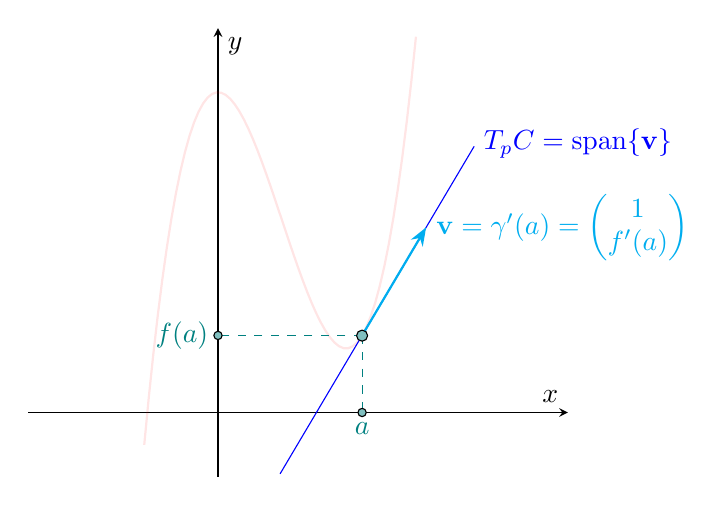
\begin{tikzpicture}
% --- Pre-calculate all values for the new function ---
\pgfmathsetmacro{\a}{2.25}              % x-coordinate of point p
\pgfmathsetmacro{\ay}{\a^3-3*\a^2+5} % y-coordinate using the new function
\pgfmathsetmacro{\slope}{3*\a^2 -6*\a} % Slope using the new derivative

\pgfmathsetmacro{\dx}{1}             % Vector x-component (made slightly smaller for visibility)
\pgfmathsetmacro{\dy}{\slope * \dx}   % Vector y-component
\pgfmathsetmacro{\endx}{\a + \dx}     % Vector end-point x
\pgfmathsetmacro{\endy}{\ay + \dy}     % Vector end-point y

% --- Pre-calculate label position for the tangent line ---
\pgfmathsetmacro{\labelx}{\a + 0.5}
\pgfmathsetmacro{\labely}{\ay + \slope*(\labelx-\a)}

\begin{axis}[
	axis lines=center,
	xlabel=$x$,xtick=\empty,
	ylabel=$y$,ytick=\empty,
	legend pos=north west,
	xmin=-2.5, xmax=5,   % Adjusted axis limits
	ymin=-1, ymax=6,    % Adjusted axis limits
	restrict y to domain=-1:6,
	axis equal, % Ensures slopes are visually correct
	clip=false,
	]
	
	% --- Plot the curve y = x^3 + x^2 + 1 ---
	\addplot[domain=-2:5, samples=100, thick, red, opacity=.1] {(x+1)*(x-2)*(x-2) + 1};
	%	\node[right, red] at (axis cs: 2.5, 2.5^3 + -3 *2.5 + 9) {Curve $C\subseteq\mathbb{R}^2$};
	%		\node[right] at (axis cs: 2.5+2, 2.5^3 + -3 *2.5 + 9) {Curve $C\subseteq\mathbb{R}^2$};
	%\addlegendentry{curve $C\subseteq\mathbb{R}^2$};
	
	% --- Plot the tangent line at x=a ---
	\addplot[domain=-2:4, samples=100, blue] {\ay + \slope*(x-\a)};
	\node[right, blue] at (axis cs:4, 4.2) {$T_pC=\mathrm{span}\{\mathbf{v}\}$};
	
	% --- Draw the tangent vector v ---
	\draw[
	-{Stealth},
	thick,
	cyan,
	] (axis cs: \a, \ay) -- (axis cs: \endx, \endy)
	node[right] {$\mathbf{v} = \gamma'(a) = \begin{pmatrix} 1\\ f'(a) \end{pmatrix}$};

	% --- Mark the point p ---
	%	\node[circle, fill=magenta, inner sep=1.5pt, label={above:$\color{magenta}p$}] at (axis cs: \a, \ay) {};
	\draw[dashed, teal] (\a,\ay) to (\a,0) node[below] {$a$};
	\draw[dashed, teal] (\a,\ay) to (0,\ay) node[left] {$f(a)$};

	\draw[fill=teal!50] (2.25,1.2) circle (2pt);
	\draw[fill=teal!50] (\a,0) circle (1.5pt);
	\draw[fill=teal!50] (0,\ay) circle (1.5pt);
\end{axis}
\end{tikzpicture}
\end{document}